%+ !TeX encoding = UTF-8
% !TeX spellcheck = fr-FR
\documentclass[a4paper,french,final]{memoir}
\usepackage{luacode}
\usepackage[german,main=french]{babel}
\usepackage[autostyle=true,maxlevel=3]{csquotes}
\usepackage{microtype}
\usepackage{fontspec}
\usepackage{geometry}
\usepackage{mathtools} 
\usepackage[math-style=french,warnings-off={mathtools-colon,mathtools-overbracket}]{unicode-math}
\setmainfont{TeX Gyre Termes}
\setmathfont{TeX Gyre Termes Math}
\setmathfont[range=bb]{STIX Two Math}
\setmathfont[range={scr,cal}]{TeX Gyre Pagella Math}
\usepackage[amsmath,thmmarks,hyperref]{ntheorem}
\usepackage[most]{tcolorbox}
\usepackage{xparse,xpatch}
\usepackage{tikz}
\usepackage{caption}
\usetikzlibrary{calc,trees,positioning,arrows,fit,shapes,calc}
\usepackage{lualatex-math}
\usepackage[unicode,naturalnames]{hyperref}
\usepackage{cleveref}
\AtBeginDocument{\let\savedemptyset\emptyset} % 
\AtBeginDocument{\let\emptyset\varnothing} % 
\AtBeginDocument{\let\savedleq\leq} % 
\AtBeginDocument{\let\savedgeq\geq} %
\AtBeginDocument{\let\leq\leqslant} % 
\AtBeginDocument{\let\geq\geqslant} %
\newcommand{\paral}{\mathrel{\!/\mkern-5mu/\!}} % \parallel existe déjà : || vs //
\makeatletter
\newcommand*{\theauthor}{\@author}
\newcommand*{\thetitle}{\@title}
\newcommand*{\thedate}{\@date}
\renewcommand{\xmapsto}[2][]{\mathrel{\mathpalette\xmapsto@{{#1}{#2}}}}
\renewcommand{\xmapsto}[2][]{\mathrel{\mathpalette\xmapsto@{{#1}{#2}}}}
\newcommand{\xmapsto@}[2]{\xmapsto@@{#1}#2}
\newcommand{\xmapsto@@}[3]{%
  \begingroup
  \sbox\z@{$\m@th#1\mathop{}\limits_{\;#2\;}^{\;#3\;}$}%
  \mathop{\Uhextensible width \wd\z@ 0 "27FC}_{#2}^{#3}%
  \endgroup
}
\renewcommand{\xLeftrightarrow}[2][]{\mathrel{\mathpalette\xLeftrightarrow@{{#1}{#2}}}}
\newcommand{\xLeftrightarrow@}[2]{\xLeftrightarrow@@{#1}#2}
\newcommand{\xLeftrightarrow@@}[3]{%
  \begingroup
  \sbox\z@{$\m@th#1\mathop{}\limits_{\;#2\;}^{\;#3\;}$}%
  \mathop{\Uhextensible width \wd\z@ 0 "027FA}_{#2}^{#3}% 027FA code for long left right double arrow in unicode-math-table.tex 
  \endgroup
}

\newcounter{proofpart}
\newcommand{\proofpart}{\@ifstar{\@proofpart}{\@@proofpart}}

\newcommand{\@proofpart}[1]{%
  \if\detokenize{#1}\relax\else{
  \par
  \addvspace{\medskipamount}%
  \noindent \itshape%
  {#1~:\par\nobreak\smallskip}%
  \normalfont
  \@afterheading
}\fi
}

\newcommand{\@@proofpart}[1]{%
  \par
  \addvspace{\medskipamount}%
  \stepcounter{proofpart}%
  \noindent Partie \theproofpart~:~\itshape%
  \if\detokenize{#1}\relax%
  \else{#1.}\fi%
  \par\nobreak\smallskip
  \normalfont
  \@afterheading
}
\makeatother
%%%%%%%%%%%%%%%%%%%%%%%%%%%%%%%%%%%%%%%%%%%%%%%%
%            NUMEROTATION (CLASSE MEMOIR)       %
%%%%%%%%%%%%%%%%%%%%%%%%%%%%%%%%%%%%%%%%%%%%%%%%%
\setsecnumdepth{subsubsection}
\renewcommand{\cftpartaftersnum}{.}
\renewcommand{\cftchapteraftersnum}{.}
\renewcommand{\cftpartdotsep}{\cftdotsep}
\renewcommand{\cftchapterdotsep}{\cftdotsep}% Chapters should use dots in ToC
\aliaspagestyle{title}{empty} 
\aliaspagestyle{part}{empty} 
%\setlength\headheight{\dimexpr \headheight+0.20004pt}

\usepackage[backend=biber,style=alphabetic]{biblatex}
\addbibresource{references.bib}
%%%%%%%%%%%%%%%%%%%%%%%%%%%%%
%   THEOREMES SANS BOITES   %
%%%%%%%%%%%%%%%%%%%%%%%%%%%%%
\theoremstyle{break}
\theoremseparator{~:} % espace fine insécable avant le :
\newtheorem{lemma}{Lemme}
\newtheorem{corollary}{Corollaire}
\newtheorem{definition}{Définition}
\theoremstyle{plain}
\newtheorem*{question}{Question}
\newtheorem*{answer}{Réponse}
\newtheorem{remark}{Remarque}
\theoremsymbol{\text{\bsc{c.q.f.d}}} % mod
\theorembodyfont{\normalfont}
\theoremprework{\setcounter{proofpart}{0}}
\newtheorem*{proof}{Démonstration}
%%%%%%%%%%%%%%%%%%%%%%%%%%%%%
%            COULEURS       %
%%%%%%%%%%%%%%%%%%%%%%%%%%%%%
\definecolor{vert}{RGB}{0,181,0}
\definecolor{oran}{RGB}{223,74,0}
\definecolor{viol}{RGB}{134,0,175}
\definecolor{roug}{RGB}{215,15,0}
\definecolor{bleu}{RGB}{0,104,180}

%%%%%%%%%%%%%%%%%%%%%%%%%%%%%
%   BOITES POUR THEOREMES   %
%%%%%%%%%%%%%%%%%%%%%%%%%%%%%
\tcbset{separator sign={},
        description delimiters parenthesis,
        label separator=-,
styletheorem/.style={enhanced,
  coltitle=black,
  colback=white,
  fonttitle=\bfseries,
  boxrule=\fboxrule,
  boxed title style={boxrule=\fboxrule},
  attach boxed title to top left={yshift=-2mm, xshift=2mm},
    }%
}
\newtcbtheorem[auto counter, number within = section]
{theoremb}{Théorème}{styletheorem,colframe=roug,
colback=white!90!roug,colbacktitle=white!80!roug,label type=theorem}{thm}
\newtcbtheorem[auto counter, number within = section]
{remarkb}{Remarque}{styletheorem,colframe=oran,
colbacktitle=white!80!oran,colback=white!90!oran,label type=remark}{rem}
\newtcbtheorem[auto counter, number within = section]
{defb}{Définition}{styletheorem,colframe=bleu,
colbacktitle=white!80!bleu,colback=white!90!bleu,label type=definition}{def}
\newtcbtheorem[auto counter, number within = section]
{noteb}{Commentaire}{styletheorem,colframe=vert,
colbacktitle=white!80!vert,colback=white!90!vert,label type=note}{note}
% le label type fait automatiquement la jonction avec cleveref pour nommer les théorèmes : le dernier groupe (thm,rem,def) permet de créer des labels automatiquement. 

%%%%%%%%%%%%%%%%%%%%%%%%%%%%%%%%%%
%  SEPARATEUR (DANS LES PREUVES) : \proofpart   %
%%%%%%%%%%%%%%%%%%%%%%%%%%%%%%%%%%%
% une  commande est définie pour séparer les preuves en deux variantes : avec et sans étoiles. (\proofpart et \proofpart*)
% Par défaut, elle crée des sous parties dans un environement de démonstration sous la forme 
% " Partie n : [titre en italique]. ", où n est un entier naturel strictement positif. Dans le cas ou le titre est vide, le point (.) n'est pas ajouté. Si le titre est vide, il faut utiliser \proofpart{}
% Avec une étoile, on obtient 
%[titre en italique : ] 

\newcommand{\deffunct}[5]{%
\begin{align*}%
      #1 \colon & #2 \to #3\\
       &#4\xmapsto{\hphantom{#1}} #5
\end{align*}%
}
%%%%%%%%%%%%%%%%%%%%%%%%%%%%%
%   PAGE DE GARDE            %
%%%%%%%%%%%%%%%%%%%%%%%%%%%%%
\newcommand{\HRule}{\rule{\paperwidth}{0.5mm}} % trait, régler eppaisseur
\newcommand*{\theuniversity}{Université de Toulon}
\newcommand*{\theyearname}{Licence de Mathématiques, parcours mathématiques, 
2\ieme~année}
\newcommand*{\thesupervisor}{Joachim \bsc{Asch}}
\author{Anastasiia \bsc{Chernetcova}~\&~Tom \bsc{Domenge}}
\title{Projet TER 2020\par
            Dénombrabilité : \par $\mathbb{N},2\mathbb{N} \ \& \ \mathbb{Q}$\par}

%%%%%%%%%%%%%%%%%%%%%%%%%%%%%%%%%%%%%%%%%%%%%%
%   Opérateurs (dans le style de max etc.   %
%%%%%%%%%%%%%%%%%%%%%%%%%%%%%%%%%%%%%%%%%%%%%%
\DeclareMathOperator{\Card}{Card} % s'utilise avec \Card en mode maths
\begin{document}
\begin{titlingpage}
\setlrmargins{*}{*}{1}
\checkandfixthelayout[nearest] 
\vspace*{\fill}%
\begin{center}
\vspace*{\fill}%
\makebox[\linewidth]{\HRule} % demande à latex l'espace pour le trait
\parbox[t]{\textwidth}{\addvspace{\parskip} % on ajoute ce qu'il faut d'espace pour sous le trait
\centering\huge\bfseries\thetitle}
 \null%Espace obligatoire pour LaTeX (boite vide) sinon l'espace est ignoré
\vspace*{\parskip}
\makebox[\linewidth]{\HRule}
\vspace*{\fill}
\diagdenomb*
\vspace{\fill}
\par \Large Rédigé par \theauthor\par Supervisé par \thesupervisor \par
\vspace*{\fill}
\large{\theyearname.\par \theuniversity, Version du \thedate}
\end{center}

\end{titlingpage}
\hypersetup{pageanchor=true}
\frontmatter
\tableofcontents
\part{Introduction}
\chapter{Avant-propos}

La notion de l'infini (noté $\infty$) apparaît pour la première fois lorsqu'on étudie l'ensemble des entiers naturels. C'est une définition intuitive de l'infini. L'infini n'est pas un nombre, il n'obéit pas aux lois usuelles $+$ et $\times$ de la même manière que les nombres réels. En mathématiques, l'une des manières les plus simples de caractériser l'infini est celle de la théorie des ensembles. L'une des propriétés principales d'un ensemble est sa taille. Comme nous allons le voir, les ensembles mathématiques peuvent être finis ou infinis : L'étude des ensembles infinis est révélatrice de paradoxes, l'un des plus célèbres  énonce qu'une partie stricte d'un ensemble infini peut contenir autant d'éléments que l'ensemble lui-même. C'est le paradoxe de l'hôtel de \bsc{Hilbert} (1924).

On peut alors se poser des questions fondamentales à l'étude de l'infini~: comment peut on caractériser les ensembles infinis ? Est-ce qu'il y a un infini << plus grand >> ou << plus petit >> que celui des nombres ?  

Dans la première partie, nous allons rappeler ce que sont les ensembles, cruciaux pour l'étude de l'infini du point de vue ensembliste.
Dans la seconde partie, nous nous consacrerons à l'étude de dénombrabilité d'ensembles usuels et aux propriétés d'ensembles dénombrables.

Notre projet devait initialement s'articuler autour de l'ouvrage~\cite{livre_ter}. Nous avons choisi une approche différente : nous voulions insister davantage sur l'aspect formel de la dénombrabilité, c'est pourquoi nous avons introduit des définitions, des notations, des propositions démontrées pour souligner notre propos. \`A notre avis, ce travail est nécessaire pour bien aborder la notion de la dénombrabilité et pour ne pas se perdre dans les différentes notions. Ainsi, nous avons choisi d'en donner une définition rigoureuse. Bien que cette notion soit intuitive, il s'avère difficile de l'expliquer rigoureusement avec des mots du langage << courant >> (non mathématique). En ce sens, le langage mathématique offre une exactitude que la langue naturelle n'a pas.

\epigraph{\foreignlanguage{german}{\enquote{\itshape Der Mathematiker abstrahiert gänzlich von der Beschaffenheit der Gegenstände und dem Inhalt ihrer Relationen; er hat es bloß mit der Abzählung und Vergleichung der Relationen unter sich zu tun}}\newline\newline
\enquote{Le mathématicien fait abstraction de la nature des objets qu'il manipule, et des relations qu'ils entretiennent ; il lui suffit de les passer en revue et de les comparer entre elles}
}{Carl~Friedrich~\bsc{Gauß}~\cite{gauss_cite}}
\mainmatter
\part{Préliminaires au dénombrement~: Comptage, applications, bijection}
\chapter{Ensembles \& applications}
\section{\'Enumération et comptage}
Avant de parler de dénombrement, il nous faut introduire la notion de comptage, car si cette notion à l'air banale et sans intérêt, elle s'avère instructive, lorsqu'il s'agit de formaliser cette notion 
Si on veut compter, à voix haute, une par une, les lettres du mot~:\[\text{cbda}\]

On le numérotera comme suit : 
\begin{table}[h]
\centering
\begin{tabular}{lllll}
c & b & d & a &  \\
1 & 2 & 3 & 4 &  
\end{tabular}
\end{table}

Ce qu'un mathématicien représentera par un \emph{diagramme sagittal,} ou \emph{patate} : 
\begin{figure}[h]
	\centering
    \begin{tikzpicture}
	\node[bullet,fill=bleu,label=left:a] (a1) at (0,4) {};    
	\node[bullet,fill=bleu,label=left:b] (a2) at (0,3) {};    
	\node[bullet,fill=bleu,label=left:c] (a3) at (0,2) {};
	\node[bullet,fill=bleu,label=left:d] (a4) at (0,1) {};%
	%
	\node[bullet,fill=roug,label=right:$1$] (b1) at (4,4) {};
	\node[bullet,fill=roug,label=right:$2$] (b2) at (4,3) {};
	\node[bullet,fill=roug,label=right:$3$] (b3) at (4,2) {};
	\node[bullet,fill=roug,label=right:$4$] (b4) at (4,1) {};%
%
	\node[fill=bleu,draw=bleu,fill opacity=0.3,fit= (a1) (a2) (a3) (a4),minimum width=2cm] (X) {} ;
	\node[fill=roug,draw=roug,fill opacity=0.3,fit= (b1) (b2) (b3) (b4),minimum width=2cm] (Y) {} ;  %
%
	\draw[->,projection] (a1) to[out=20, in=150] (b4);
	\draw[->,projection] (a2) to[out=20, in=160] (b2);
	\draw[->,projection] (a3) to[out=20, in=170] (b1);
	\draw[->,projection] (a4) to[out=20, in=150] (b3);
%
	\draw[|->,thick,shorten <=1cm,shorten >=1cm] (X.north) -- node [midway,above,align=center]{comptage} (Y.north);
%	\node[below] at (X.south) {t};
	\end{tikzpicture}%
%
	\caption{diagramme sagittal représentant le comptage ci-dessus.}
	\label{fig:comptage}
\end{figure}
%
%\diagfonctinj
%\diagfonctsurj

%\diagcompfonct
Si cet exemple a l'air simple, il n'est pas simpliste pour autant :  ce procédé, qui consiste à associer à chaque lettre un nombre est omniprésent en mathématiques et il porte le nom \emph{d'application}.
Plus remarquable encore, ce diagramme permet même de donner une première définition quasi-formelle de ce qu'est une application. Une chose est \emph{cruciale} : chaque lettre ne doit être comptabilisée une seule et unique fois, sinon, le résultat final est faussé ! 

Pour fixer les idées voici deux nouvelles applications.

	\begin{figure}[H]
	\centering
    \begin{tikzpicture}
	\node[bullet,fill=bleu,label=left:$1$] (a1) at (0,4) {};    
	\node[bullet,fill=bleu,label=left:$2$] (a2) at (0,3) {};    
	\node[bullet,fill=bleu,label=left:$3$] (a3) at (0,2) {};
	\node[bullet,fill=bleu,label=left:$4$] (a4) at (0,1) {};%
	%
	\node[bullet,fill=roug,label=right:pair] (b1) at (4,4) {};
	\node[bullet,fill=roug,label=right:impair] (b2) at (4,3) {};
%
	\node[fill=bleu,draw=bleu,fill opacity=0.3,fit= (a1) (a2) (a3) (a4),minimum width=2cm] (X) {} ;
	\node[fill=roug,draw=roug,fill opacity=0.3,fit= (b1) (b2),minimum width=3.2cm] (Y) {} ;  %
%
	\draw[->,projection] (a1) to[out=20, in=140] (b2);
	\draw[->,projection] (a2) to[out=20, in=160] (b1);
	\draw[->,projection] (a3) to[out=20, in=140] (b2);
	\draw[->,projection] (a4) to[out=20, in=160] (b1);
%
	\draw[|->,thick,shorten <=1cm,shorten >=1cm] (X.north) -- node [sloped, anchor=center, midway,above,align=center]{parité} (Y.north);
%	\node[below] at (X.south) {t};
	\end{tikzpicture}%
%
	\caption{application parité.}
	\label{fig:parité}
\end{figure}	

Cet exemple simple est très utilisé, notamment en informatique, en remplaçant pair et impair par $0$ et $1$, respectivement. \sidepar{les développeurs aguerris auront reconnu la formule ~\textup{\texttt{n=n\&1}}.}

\hrulefill
\begin{figure}[htb]
	\centering
    \begin{tikzpicture}
	\node[bullet,fill=bleu,label=left:lundi] (a1) at (0,4) {};    
	\node[bullet,fill=bleu,label=left:mardi] (a2) at (0,3) {};    
	\node[bullet,fill=bleu,label=left:mercredi] (a3) at (0,2) {};
	\node[bullet,fill=bleu,label=left:jeudi] (a4) at (0,1) {};%
	\node[bullet,fill=bleu,label=left:vendredi] (a5) at (0,0) {};%
	\node[bullet,fill=bleu,label=left:samedi] (a6) at (0,-1) {};%
	\node[bullet,fill=bleu,label=left:dimanche] (a7) at (0,-2) {};%

	%
	\node[bullet,fill=roug,label=right:$0$] (b1) at (4,4) {};
	\node[bullet,fill=roug,label=right:$1$] (b2) at (4,3) {};
	\node[bullet,fill=roug,label=right:$2$] (b3) at (4,2) {};
	\node[bullet,fill=roug,label=right:$3$] (b4) at (4,1) {};%
	\node[bullet,fill=roug,label=right:$4$] (b5) at (4,0) {};%
	\node[bullet,fill=roug,label=right:$5$] (b6) at (4,-1) {};%
	\node[bullet,fill=roug,label=right:$6$] (b7) at (4,-2) {};%

%
	\node[fill=bleu,draw=bleu,fill opacity=0.3,fit= (a1) (a2) (a3) (a4) (a5) (a6) (a7),minimum width=4.6cm] (X) {} ;
	\node[fill=roug,draw=roug,fill opacity=0.3,fit= (b1) (b2) (b3) (b4) (b5) (b6) (b7),minimum width=2cm] (Y) {} ;  %
%
	\draw[->,projection] (a1) to[out=20, in=150] (b7);
	\draw[->,projection] (a2) to[out=20, in=160] (b2);
	\draw[->,projection] (a3) to[out=20, in=170] (b3);
	\draw[->,projection] (a4) to[out=20, in=150] (b4);
	\draw[->,projection] (a5) to[out=20, in=150] (b5);
	\draw[->,projection] (a6) to[out=20, in=150] (b6);
	\draw[->,projection] (a7) to[out=20, in=150] (b1);
%
	\draw[|->,thick,shorten <=1cm,shorten >=1cm] (X.north) -- node [sloped, anchor=center, midway,above,align=center]{jour n\textsuperscript{o}} (Y.north);
%	\node[below] at (X.south) {t};
	\end{tikzpicture}%
%
	\caption{ Application \enquote{jours de la semaine} (convention anglo-saxonne).}
	\label{fig:jourssem}
\end{figure}
\sidepar{ En 1990, \bsc{Keith} a trouvé le jour correspondant à une date grâce à l'expression suivante (en  langage \textup{\textsf{C}) :\\\texttt{int weekday  = (d~+=~m~<~3~? y-\/-~: y - 2, 23*m/9 + d + 4 + y/4- y/100 + y/400)\%7;  
	}}}
\clearpage
\section{Étude de deux cas limites}
Il y a cependant un détail à régler : Comment considère-t-on les points qui ne sont pas reliés ?
\begin{figure}[h]
	\centering
    \begin{tikzpicture}
	\node[bullet,fill=bleu,label=left:a] (a1) at (0,4) {};    
	\node[bullet,fill=bleu,label=left:b] (a2) at (0,3) {};    
	\node[bullet,fill=bleu,label=left:c] (a3) at (0,2) {};
	\node[bullet,fill=bleu,label=left:d] (a4) at (0,1) {};
	\node[bullet,fill=bleu,label=left:e] (a5) at (0,0) {};

	%
	\node[bullet,fill=roug,label=right:$1$] (b1) at (4,4) {};
	\node[bullet,fill=roug,label=right:$2$] (b2) at (4,3) {};
	\node[bullet,fill=roug,label=right:$3$] (b3) at (4,2) {};
	\node[bullet,fill=roug,label=right:$4$] (b4) at (4,1) {};%
%
	\node[fill=bleu,draw=bleu,fill opacity=0.3,fit= (a1) (a2) (a3) (a4) (a5),minimum width=2cm] (X) {} ;
	\node[fill=roug,draw=roug,fill opacity=0.3,fit= (b1) (b2) (b3) (b4),minimum width=2cm] (Y) {} ;  %
%
	\draw[->,projection] (a1) to[out=20, in=150] (b4);
	\draw[->,projection] (a2) to[out=20, in=160] (b2);
	\draw[->,projection] (a3) to[out=20, in=170] (b1);
	\draw[->,projection] (a4) to[out=20, in=150] (b3);
%
	\draw[|->,thick,shorten <=1cm,shorten >=1cm] (X.north) -- node [sloped, anchor=center, midway,above,align=center]{1\ier~cas} (Y.north);
%	\node[below] at (X.south) {t};
	\end{tikzpicture}%
%
	\caption{Un point n'est pas relié à gauche. Est-ce une application ?}
	\label{fig:comptinj}
  \end{figure}
  %\clearpage
  Revenons au problème de comptage. On se trouverait dans la situation suivante
\begin{table}[h]
\centering
\begin{tabular}{llllll}
c & b & d & a & e \\
1 & 2 & 3 & 4 & \textcolor{red}{?}
\end{tabular}
On a oublié la lettre e !

Le cas de la ~\cref{fig:comptinj} n'est pas satisfaisant. Ce n'est pas une application.

\hrulefill
\end{table}
\begin{figure}[h]
	\centering
    \begin{tikzpicture}
	\node[bullet,fill=bleu,label=left:a] (a1) at (0,4) {};    
	\node[bullet,fill=bleu,label=left:b] (a2) at (0,3) {};    
	\node[bullet,fill=bleu,label=left:c] (a3) at (0,2) {};
	\node[bullet,fill=bleu,label=left:d] (a4) at (0,1) {};%
 	%
	\node[bullet,fill=roug,label=right:$1$] (b1) at (4,4) {};
	\node[bullet,fill=roug,label=right:$2$] (b2) at (4,3) {};
	\node[bullet,fill=roug,label=right:$3$] (b3) at (4,2) {};
	\node[bullet,fill=roug,label=right:$4$] (b4) at (4,1) {};%
	\node[bullet,fill=roug,label=right:$5$] (b5) at (4,0) {};%
%
	\node[fill=bleu,draw=bleu,fill opacity=0.3,fit= (a1) (a2) (a3) (a4),minimum width=2cm] (X) {} ;
	\node[fill=roug,draw=roug,fill opacity=0.3,fit= (b1) (b2) (b3) (b4) (b5),minimum width=2cm] (Y) {} ;  %
%
	\draw[->,projection] (a1) to[out=20, in=150] (b4);
	\draw[->,projection] (a2) to[out=20, in=160] (b2);
	\draw[->,projection] (a3) to[out=20, in=170] (b1);
	\draw[->,projection] (a4) to[out=20, in=150] (b3);
%
	\draw[|->,thick,shorten <=1cm,shorten >=1cm] (X.north) --node [sloped, anchor=center, midway,above,align=center]{2\ieme~cas} (Y.north);
%	\node[below] at (X.south) {t};
	\end{tikzpicture}%
%
	\caption{Un point n'est pas relié à droite. Est-ce une application ?}
	\label{fig:fonctcomp}
  \end{figure}
\clearpage
 Revenons une fois encore au comptage de mots pour trancher. Dans ce cas, on obtient :
\begin{table}[h]
\centering
\begin{tabular}{llllll} 
c & b & d & a & \texttt{\backslash0} \\
1 & 2 & 3 & 4 &  5
\end{tabular}
\end{table} 
\sidepar{\vspace*{-4\onelineskip}Le \textup{\texttt{\backslash0}} signale la fin d'un mot ou d'une chaîne de caractères (caractère 0 en \hyphenation{ASCII} ASCII)}
Contrairement au cas précédent, nous avions correctement compté le nombre de lettre du mot. On a simplement une valeur surnuméraire.  On peut donc sans risque accepter ce cas particulier. Comme toutes les valeurs ne sont pas atteintes, on dira que l'application est \emph{non-surjective}.

\section{Formalisation du concept d'application}
Maintenant que l'on dispose d'une idée claire du concept d'application, on va essayer de le formaliser. En fait, une fonction se décrit à l'aide de 3 éléments :
\begin{enumerate}
  \item
		Un ensemble dit \emph{de départ}, en \textcolor{bleu}{bleu} dans nos diagrammes.
  \item
		Un ensemble dit \emph{d'arrivée}, en \textcolor{roug}{rouge} dans nos diagrammes.
  \item
		Un ensemble de \emph{flèches} qui relient un élément de l'ensemble de départ à un élément de l'ensemble d'arrivée.
\end{enumerate}
La \cref{fig:comptinj} nous a apporté une précision supplémentaire :

\begin{center} % Center the box
  \fbox{% creates the frame
  \parbox{\dimexpr\linewidth-2\fboxsep-2\fboxrule}% An \fbox has the width of its contents plus 2 \fboxsep plus 2 \fboxrule
  {\centering \textbf{Tout} élément de l'ensemble de départ est relié à \textbf{un seul} élément de l'ensemble d'arrivée.}%
  } %Creates the text, centered with centering
\end{center}
Pour formaliser la fonction de flèche, on utilise les couples : ce sont des \emph{paires ordonnées} d'objets. Ainsi, par exemple, dans la \cref{fig:fonctcomp}, la flèche $b\to 2$ peut être réprésentée par le couple $(b;2)$.
\noindent On choisit par la suite de représenter une flèche $\text{départ}\to \text{arrivée}$ par le couple $(\text{départ};\text{arrivée})$.

Nous sommes désormais en capacité de formaliser la notion d'application :
\begin{defb}{Application, graphe}{app}
  Soit $X$ et $Y$ deux ensembles quelconques.

  On appelle \emph{application de $X$ dans $Y$} le triplet $f\eqdef(X,Y,F)$, où $F\subseteq (X\times Y)$ \footnote{ \textit{litt.} $F$, un ensemble de couples} vérifie : \[ \boxed{\forall x \in X, \exists!\,y \in Y \mid (x,y) \in F.\,}\footnote{C'est la condition encadrée plus haut.}\]
  L'ensemble $F$ est appelé \emph{graphe de l'application} $f$, On le notera $\mathscr{G}_{f}$.
 \end{defb}
\chapter{Applications injectives \& surjectives, composition}
\chapter{Définition de la cardinalité}
\section{Ensembles finis et infinis}

\begin{defb}{Finitude}{fini}
     Soit $E$ un ensemble. 
	    
	On dit que $E$ est fini si $E = \emptyset$ ou s'il existe une bijection $\phi~: \{1,\dots,n \} \to E$, avec $n \in \NN$.

	Dans ce cas, on dit que $E$ est de cardinal $n$ (ou de puissance $n$), et on note le cardinal $\Card(E)$. 
\end{defb} 

%\sidepar{\vspace{-6\baselineskip}Quelle est la puissance d'un coton-tige ? \\ -Deux ouates.}

\begin{defb}{\'Equipotence}{equip}
    On dit que $E$ et $F$ sont équipotents s' il existe $\phi~: E \to F$ bijective. Dans ce cas, on note $E \mathrel{\approx} F$. 
\end{defb}

\begin{theoremb}{}{mmpuiss}
    $ \mathrel{\approx}$ est une relation d'équivalence. 
\end{theoremb}
\begin{proof}\sidepar{Une relation d'équivalence est un \enquote{prisme de lecture} mathématique.
\\[\onelineskip]
Deux ensembles de même cardinalité ont même valeur à nos yeux, on les met donc dans le même panier, ou plutôt, dans la même classe\textellipsis}
    Soient $E, F, G$, trois ensembles.
	\begin{enumerate} 
		\item $E \mathrel{\approx} E$, car l'application identité est une bijection. $\mathrel{\approx}$ est réflexive.
		\item $E \mathrel{\approx} F$ signifie qu'il existe une bijection de E dans F. Alors, l'inverse de cette bijection est une application de F dans E, elle-même bijective.
		\item Si $E \mathrel{\approx} F$ et $F \mathrel{\approx} G$ alors il existe une bijection de E dans F, $\phi$, et une bijection de F dans G, $\psi$. Par composition, $\psi\circ\phi$ est une bijection de E dans G, c. -à-d. $E \mathrel{\approx} G$. $\mathrel{\approx}$ est transitive. 
	\end{enumerate}
	$\mathrel{\approx}$ est bien une relation d'équivalence.
\end{proof}

\begin{theoremb}{}{assequiv}
	Soient $E, F$ deux ensembles \textbf{finis} et $\phi~: E \to F$ une application. Si $E \mathrel{\approx} F$ alors les 3 assertions suivantes sont équivalentes~:
	
	\begin{enumerate}
		\item $\phi$ est injective ;
		\item $\phi$ est surjective ;
		\item $\phi$ est bijective. 
	\end{enumerate}
\end{theoremb}

\begin{defb}{Ensemble infini}{ifini}
	Soit $E$ un ensemble.
	
	On dit que $E$ est infini ssi $E$ n'est pas fini.
\end{defb}

\begin{theoremb}{}{partn} 
	Toute partie de $\NN$ est finie ssi elle est majorée. 
\end{theoremb}



\begin{theoremb}{}{ninfini}
	$\NN$ est infini. 
\end{theoremb}


\begin{proof}
	Si $\NN$ était fini, d'après le \cref{thm:partn}, $\NN$ admettrait un majorant. Autrement dit \[\exists k \in \NN, \forall x \in \NN, x \leq k.\]

	Or la construction de $\NN$ implique que si $ k \in \NN$, alors $k + 1 \in \NN$ et $\exists x \in \NN, x > k, x= k+1$, d'où une contradiction. 
	
	Donc $\NN$ est infini.
\end{proof}
\section{Des parties infinies ?}
L'intuition nous pousse à croire que, comme dans le cas fini, toute partie de $\NN$, stricte, est finie. Il n'en est rien, comme Euclide l'a démontré, vers~-300~av.~J.C. 

On se propose donc ici de reformuler sa démonstration en terme modernes. 
\begin{defb}{Divisibilité}{div}
Soit $a,b$ deux entiers naturels. On dit que $a$ \emph{divise} $b$ ou que $b$ est un \emph{multiple} de $a$, et on note $a\mid b$, s'il existe un entier naturel $k$ tel que : $$b=ka \xLeftrightarrow{ a \mathrel{\neq} 0 } \frac{b}{a}=k.$$
\end{defb}
\begin{remarkb}{}{divinf}
0 ne divise que 0. De plus, si $a$ divise $b$, alors $a\leq b$. Par conséquent, 1 est le seul entier naturel qui divise 1.
\end{remarkb}
\begin{defb}{Nombre premiers entre eux}{coprem}
On dit que deux nombres entiers $n,p$ sont \emph{premiers entre eux} ou \emph{copremiers} s'ils n'ont pas de diviseur commun, mis à part 1. On dit alors que $n$ \emph{est premier} à ou avec $q$.
\end{defb}
\begin{defb}{Nombre premier}{prem}
On dit qu'un nombre est premier, s'il n'a pas de diviseurs autre que 1 et lui-même. Dans le cas contraire, on le dit \emph{composé}.

Par convention\footnotemark, 1 n'est ni premier ni composé.
\end{defb}
 \footnotetext{Cette convention est récente dans l'histoire des mathématiques : 1 était considéré premier jusqu'à la fin du XIX\ieme~siècle, voire au début du XX\ieme.}
La remarque suivante justifie l'emploi du même vocabulaire : 
\begin{remarkb}{}{prem-equiv}
Un nombre est premier si et seulement s'il est copremier avec tous ceux qui le précèdent, c'est-à-dire s'il n'a aucun diviseur commun avec un entier qui lui est inférieur. 
\end{remarkb}
\begin{lemmab}{}{divprod}
Si $n$ divise deux entiers $a,b$, il divise aussi leur produit $ab$. 
\end{lemmab}
\begin{proof}
Comme $n$ divise $a$, il existe un entier $k$ tel que $a=kn$, de même, comme $n$ divise $b$, il existe un entier $k'$ tel que $b=k'n$. Ainsi, \[ab=\underbrace{knk'}_{\eqdef k_2\in \mathbb{N}}{}\times n.\]
\end{proof}
Le lemme suivant est \textbf{fondamental} dans ce qui suit :
\begin{lemmab}{Théorème fondamental de l'arithmétique}{Fonda-Arith}
  Tout entier naturel non-nul peut être écrit comme un produit de nombres premiers d'une unique façon, à l'ordre près des facteurs.
\end{lemmab}
La démonstration de ce théorème est rejetée en~\cref{annexe:thmfondarith}.

Ces rappels balayés, on peut démontrer le résultat d'Euclide 

\begin{theoremb}{Infinité des nombres premiers}{nombpreminf} 
Toute liste finie de nombre premiers est nécessairement incomplète.

Autrement dit, il existe une infinité de nombres premiers.
\end{theoremb}
\begin{proof}
\reversemarginpar
On démontre le résultat par récurrence. Une liste vide (à 0 éléments) ne contient aucun nombre premier, elle est donc incomplète car 2 est premier. 
Supposons que l'on dispose d'une liste finie de $n$ nombres premiers, pour $n$ un entier naturel quelconque. En triant notre liste dans l'ordre croissant, on obtient une suite de $n$ entiers, que l'on note $(p_i)_{i\in \left\lBrack1;n\right\rBrack}$. Alors,on peut considérer, l'entier $N$ défini par : \[ N=\prod_{i=1}^{n} p_i\]\sidepar{\vspace*{-3.5\baselineskip}\itshape \footnotesize Donc $N$ est égal à Pi de 1 à $n$ de $p_i$}
Si notre suite est vide, on pose $N=2$.

Les termes $(p_i)_{i\in \left\lBrack1;n\right\rBrack}$ sont les facteurs premiers de $N$, par le \cref{lem:Fonda-Arith}.
\sidepar{\itshape \footnotesize $2$ est le plus petit nombre premier.}
Si $N+1$ est premier, alors notre liste est incomplète. Dans le cas contraire, on est assuré de l'existence d'un facteur premier $p$ pour $N+1$. Mais, d'après le \cref{lem:ncopremsn}, ce facteur premier n'est pas dans la décomposition de $N$, il n'est donc pas dans notre liste. Dans les deux cas, notre liste est incomplète. 
\end{proof}
Comme on l'a vu ci-avant, l'infini nous réserve quelques surprises. Il est donc judicieux de considérer une famille plus large d'ensemble : les ensembles \emph{dénombrables} et \emph{au plus dénombrables}. 
\part{Dénombrabilité}
\chapter{\texorpdfstring{\'Etude de 2$\NN$, $\ZZ$, $\QQ$}{Dénombrabilité : Étude de N,2N,Z, et Q}} 
\section{Introduction : le paradoxe de Hilbert}

Si on définit l'infini comme la cardinal de $\NN$, quel est le cardinal de $E= \{-1, 0, 1, 2, \dots\}$ ? Intuitivement on se dit que $E$ est infini, mais est-il plus grand que $\NN$ ? Il nous manque un moyen de comparer les infinis.

Pour introduire le problème d'une manière concrète, on peut avoir recours au paradoxe de l'hôtel de Hilbert. Imaginons qu'on ait un hôtel avec une infinité de chambres numérotées par les entiers naturels. Les chambres sont toutes occupées. On place un hôte par chambre. Cependant, si un nouveau client arrive, il suffit que l'hôtelier, fin mathématicien, demande au client dans la chambre $n$ de se déplacer dans la chambre $n+1$ (le client présent dans la chambre 0 peut aller dans la chambre 1, le client présent dans la chambre 1 va dans la chambre 2, \dots) Le nouveau client peut s'installer dans l'hôtel.

Imaginons maintenant qu'une infinité de nouveaux clients arrive à l'hôtel. Pour les accueillir, l'hôtelier peut demander au client dans la chambre $n$ d'aller dans la chambre $2n$. Ainsi toutes les chambres portant un numéro impair sont libérées et tous les nouveaux clients sont logés.

Ce paradoxe introduit des résultats contre-intuitifs quant à la cardinalité de $2 \NN$ et de sous-ensembles de $\NN$ que l'on va démonter d'une manière plus formelle.

\begin{figure}[htb]
    \centering
    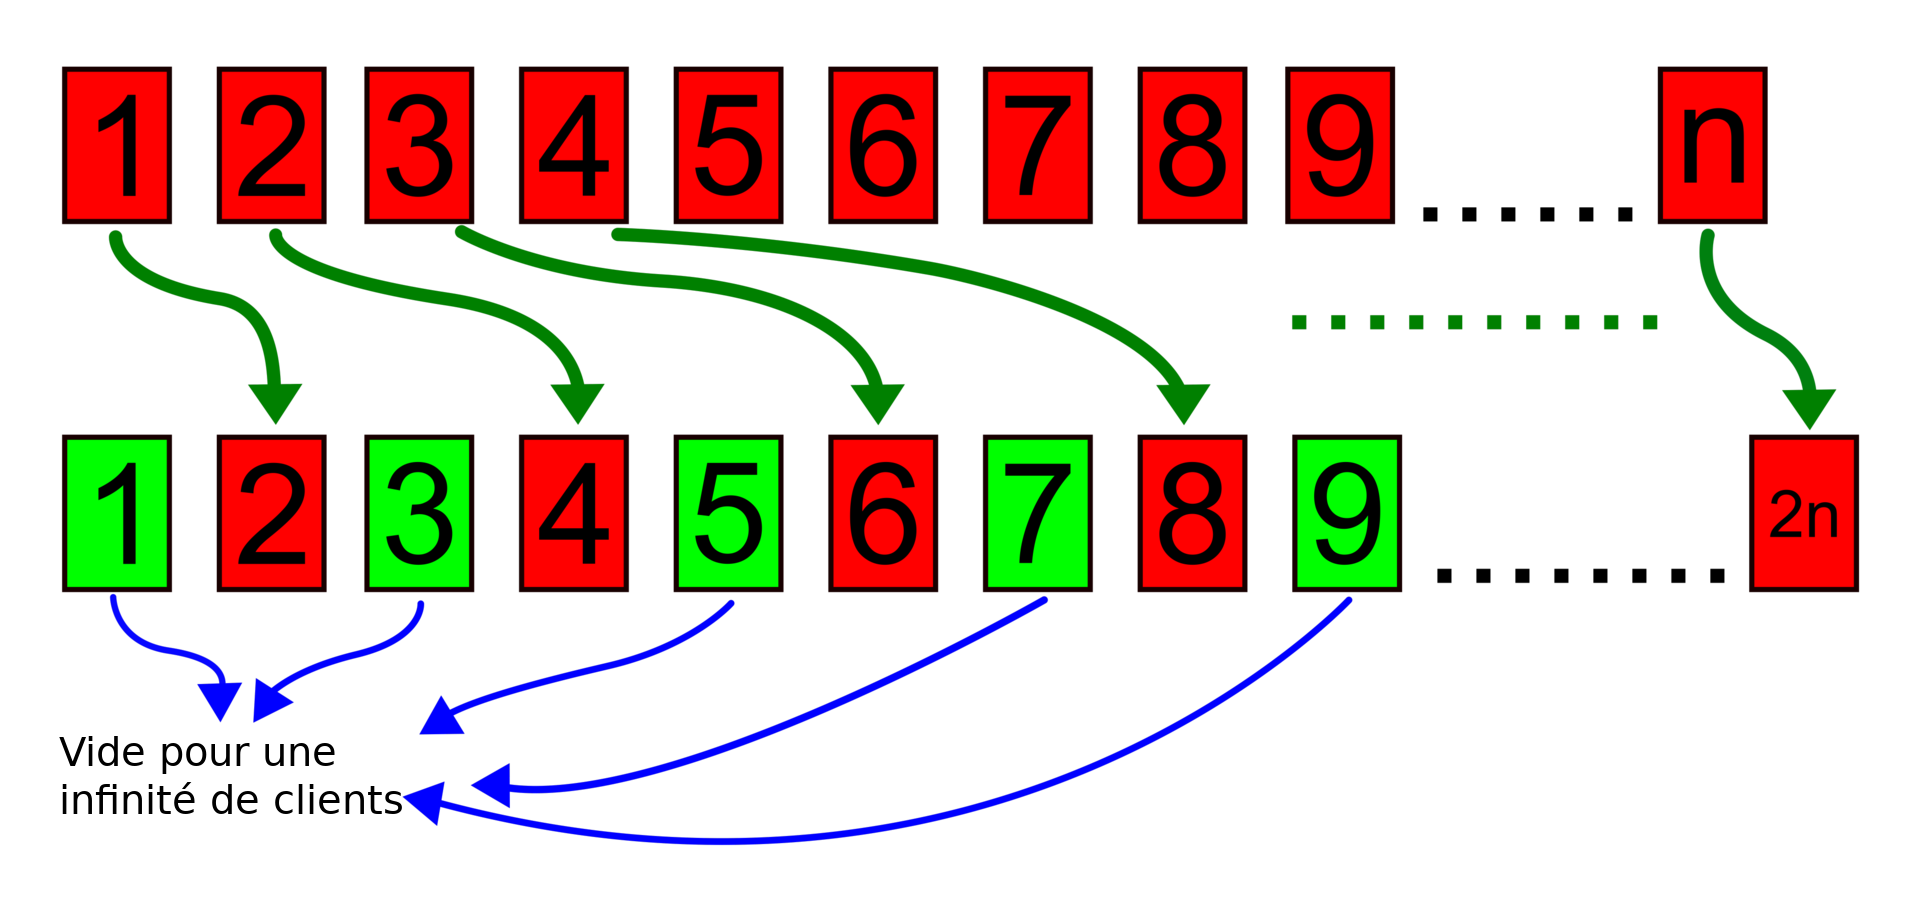
\includegraphics[width=0.7\textwidth,keepaspectratio]{hotel de hilbert.png}
    \caption{Hôtel de Hilbert}
    \label{fig:hotel_hilbert}
\end{figure}
\clearpage
\section{Définition générale de la dénombrabilité}
Commençons par une définition précise de ce que l'on vient de constater :
\begin{defb}{Ensemble démombrable, au plus dénombrable}{denomb}

	 Soit $E$ un ensemble infini. 
	 
	 On dit que $E$ est dénombrable ssi il existe une application $\phi~: \NN \to E $ bijective. 
	 
	 Un ensemble fini ou dénombrable est dit au plus dénombrable. \newline
	 On note par la suite $\aleph_0$, lire \emph{alèf zéro}\footnotemark, le cardinal de $\NN$. 
\end{defb}
\footnotetext{Aleph, première lettre  de l'alphabet hébreu}


\section{\texorpdfstring{Dénombrabilité de 2$\NN$}{Dénombrabilité de 2N}}
\label{sec:denombrabilite_usuelle}
Il semble que l'ensemble des nombre premier n'est pas le seul à défier notre intuition :  voici un résultat sur la dénombrabilité de  $2\NN$, l'ensemble des entiers naturels pairs.

\begin{theoremb}{Dénombrabilité de 2$\NN$}{}
	L'ensemble 2$\NN$ des entiers naturels pairs est dénombrable. 
\end{theoremb}

\begin{proof}
	On construit l'application \[ \begin{array}{cccc}
	\ & \NN& \to& 2\NN \\
	\phi~: & n & \mapsto & 2n
	\end{array}.\]
	
	Cette application $\phi $ est bijective car sa réciproque est $ \phi^{-1}~: \begin{array}{ccc}
	2\NN & \to & \NN\\
	k & \mapsto & \frac{k}{2}
	\end{array}$. 
	
	2$\NN$ est en bijection avec $\NN$. 2$\NN$ est bien un ensemble dénombrable de cardinal $\aleph_0$. 
\end{proof}

On peut introduire un résultat plus général qui couvre toute partie de $\NN$. 

\begin{theoremb}{Dénombrabilité des parties infinies de $\NN$}{}
	Toute partie $E \subset \NN$ infinie a le même cardinal que $\NN$. 
\end{theoremb}

\begin{proof}
	On construit, par récurrence, une bijection $\phi~: \NN \to E$ telle que: 
	
	\[\left\lbrace \begin{array}{c}
	\phi(0) = \min \{x \in E\} \\
	\forall n \in \NN, \phi(n+1) = \min \{x \in E, x > \phi(n) \}
	\end{array} \right.\]
	
	C'est bien une bijection~: elle est injective et surjective car $\forall k \in \NN, k \leq \phi(k)$. 
\end{proof}
On en déduit le résultat suivant : 
\begin{theoremb}{}{parties}
	Soient $E$ et $F$ deux ensembles. 
	Si $E \subset F$ et si $F$ est dénombrable, alors $E$ est au plus dénombrable.
\end{theoremb}
\section{\texorpdfstring{Dénombrabilité de $\NN^2$}{Dénombrabilité de N²}}
Pour un ensemble $E$ fini de cardinal $n$, à moins que $\Card(E) = 1$, $\Card(E^2) \neq \Card(E)$. On pourrait penser que $\NN^2 $ contient plus d'élements que $\NN$. 

\begin{theoremb}{Dénombrabilité de $\NN^2$}{n2_denombrable}
	$\NN^2$ est dénombrable. 
\end{theoremb}

\begin{proof} 
	On peut compter les couples $(n,m) \in \NN^2$ comme suit~: \par On représente ces couples sur un quart de plan cartésien. 
	On part du couple $(0, 0)$. Dans la ligne suivante, on range $(1,0) $ et $(0,1)$. On continue avec $(2,0), (1,1), (0,2)$ (on parcourt la diagonale du point de coordonnées $(n,0)$ pour arriver au point de coordonnées $(0,n)$). Ce procédé est illustré dans la  \cref{fig:n_croix_n}.
	\begin{figure}[htb]
		\centering
		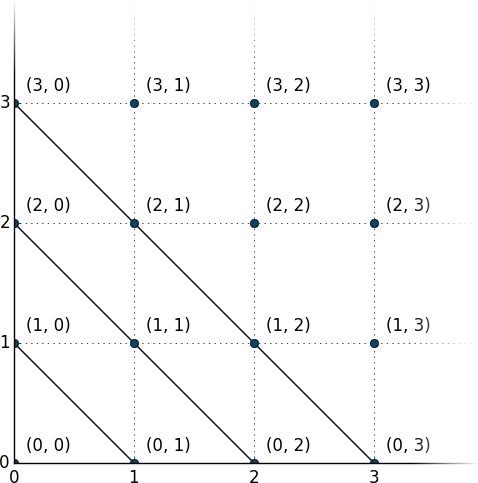
\includegraphics[scale=0.3]{n_croix_n.png}
		\caption{Dénombrabilité de $\NN^2$}
		\label{fig:n_croix_n}
	\end{figure}
	
	On obtient la séquence suivante~:
	
	\[\begin{array}{l}
		(0,0) \\
		(1,0), (0,1) \\
		(0,2), (1,1), (2,0) \\
		(3,0), (1,2), (2,1), (0,3) \\
		\cdots
	\end{array}.\]
	Plus formellement, l'application qui range les couples de cette manière est 
	\[\begin{array}{cccc}
		\ & \NN \times \NN & \to & \NN \\
		\phi~: & (n,m) & \mapsto & {\underbrace{\frac{(n+m)(n+m+1)}{2}}_{\text{la place du couple dans la ligne}}} +  {\underbrace{\vphantom{\frac{(n+m)(n+m+1)}{2}} m}_{\text{la place du couple dans la colonne}}}
	\end{array}.\]
	
	
	$\phi$ est bien bijective. $\NN^2$ est bien dénombrable.
\end{proof}


Par récurrence sur $k \in \NN$, on peut montrer le théorème suivant :
\begin{theoremb}{}{nk_denombrable}
    $\NN^k$ est dénombrable.
\end{theoremb}

\begin{proof}

Pour $k = 3$, on peut, en utilisant les notations du \cref{thm:n2_denombrable}, établir une bijection entre $\NN^2$ et $\NN^3$. Posons $h_3 : \NN^2 \to \NN^3$ telle que $h_3(n,m) = (n,\phi^{-1}(m))$. $h_3$ est bien une bijection. 

Soit $k \in \NN$ fixé. Supposons l'hypothèse vraie au rang $k$, i. e. $\NN^k$ est dénombrable.

On construit une bijection entre $\NN^2$ et $\NN^{k+1}$. On pose $h_{k+1}(n_1, \dots, n_{k+1}) = (h_k(n_1, \dots, n_k),n_{k+1})$ où $h_k(n_1, \dots, n_k) \in \NN$ car d'après l'hypothèse de récurrence, $\NN^k$ est dénombrable. On a ainsi établi une bijection entre $\NN^{k+1}$ et $\NN^2$. Or $\NN^2$ est dénombrable. Donc $\NN^k$ est dénombrable. 

Par récurrence, $\forall k \in \NN, \NN^k$ est dénombrable. 

\end{proof}
De la dénombrabilité de $\NN^2$, on peut démontrer le théorème suivant :. 
\begin{theoremb}{Produit cartésien d'ensembles dénombrables}{cartesien}
	Soient $A, B, A_1, \dots, A_i, \dots, A_n$ des ensembles dénombrables. 
	\begin{enumerate}
		\item Le produit cartésien $A \times B$ est dénombrable. 
		\item Plus généralement, tout produit \textbf{fini} $\prod_{i=1}^{n} A_i $ est dénombrable.
	\end{enumerate}
\end{theoremb}
\begin{proof}
	Si $E$ et $F$ sont dénombrables, il existe $\phi~: E \to \NN$ et $\psi~: F \to \NN$ bijectives. On peut alors définir \[ \begin{array}{cccc}
	\ & A \times B & \to & \NN^2 \\
	f~: & (x,y) & \mapsto & (\phi(x), \psi(y))
	\end{array}.\]
	
\end{proof}

$f $ est bien bijective. Donc $A \times B$ est bien dénombrable. On procède par récurrence immédiate pour $k$ ensembles. 

Soit $\prod_{i =1}^k A_i$ le produit cartésien de $k$ ensembles dénombrables. Si $\forall i \in \{1,\dots,k\}, \phi_i : A_i \to \NN$ est une bijection, alors on peut construire l'application \[ \begin{array}{cccc}
	\ & \prod_{i=1}^k A_i & \to & \NN^k\\
	f~: & (x_1,\dots,x_k) & \mapsto & (\phi_1(x_1),\dots, \phi_k(x_k))
	\end{array}.\] 
C'est une bijection de $\prod_{i=1}^k A_i $ vers $\NN^k$ qui est dénombrable. Donc $\prod_{i=1}^kA_i$ est dénombrable.


On peut encore montrer le résultat suivant : 
\begin{theoremb}{Union de deux ensembles dénombrables}{union}
    Soit $(A_i)_{i \in I}$ une famille dénombrable d'ensembles dénombrables. 
	Alors $A= \bigcup_{i \in I} A_i$ est dénombrable. 
\end{theoremb} 
\begin{proof}
	En effet, on peut écrire $\forall i \in I, A_i = \{x_{n,i}, n \in \NN\}$. Chaque élement $x_{n, i}$ est indéxé par sa position $n$ dans $A_i$ et la position $i$ de $(A_i)$ dans $I$. 
	
	Ainsi $A = \bigcup_{i \in I} A_i = \{x_{n, i}, (n,i) \in \NN \times I\}$. Les élements $x_{n,i}$ sont indéxés par $\NN \times I$ qui est un produit cartésien d'ensembles dénombrables ($I$ est une famille indéxée par $\NN$, elle est bien dénombrable). Donc $A$ est dénombrable.
\end{proof}
\section{\texorpdfstring{Dénombrabilité de $\ZZ$ et de $\QQ$}{Dénombrabilité de Z et Q}}

Intuitivement on pourrait penser que l'ensemble des entiers $\ZZ$ a un cardinal supérieur à $\NN$ étant donné qu'il contient ``deux fois plus" d'élements~: les entiers naturels et les entiers négatifs. 

\begin{theoremb}{Dénombrabilité de $\ZZ$}{denz}
	L'ensemble $\ZZ$ des entiers est dénombrable. 
\end{theoremb}

\begin{proof}
L'idée de la démonstration revient à écrire l'ensemble des entiers, dans l'ordre suivant~:  $\ZZ=\left\lbrace 0,1,(-1),2,(-2),3,(-3) \dots\right\rbrace$ 

	Pour montrer que le cardinal de $\ZZ$ est bien $\aleph_0$, on définit donc l'application $\phi~: \NN \to \ZZ$ telle que \[ \forall k \in \NN, \
	\begin{dcases}
	\phi(2k)& = -k \\
	\phi(2k + 1)& = k+1
	\end{dcases}
\]
	C'est bien une bijection. Donc $\ZZ$ est dénombrable. 
\end{proof}
\begin{theoremb}{Dénombrabilité de $\QQ$}{denq}
	$\QQ$ est dénombrable.
\end{theoremb}
\begin{proof}
	Tout $x \in \QQ$ a un unique représentant irréductible $\frac{p}{q}$ où $p \wedge q = 1$. 
	
	Pour établir une bijection entre $\QQ$ et $\NN$, on commence par écrire un tableau où on range $\frac{p}{q}$ à la colonne $q$ et à la ligne $p$.  
	
	On parcourt le tableau comme c'est indiqué par les flèches dans la \cref{fig:denombQ}. 
	
	On part de $\frac{1}{1}$ dans le tableau. On se déplace à la colonne suivante pour atteindre $\frac{1}{2}$. On parcourt le tableau diagonalement vers le bas pour atteindre $\frac{2}{1}$, on descend d'une case pour obtenir $\frac{3}{1}$ et on parcourt le tableau en diagonale vers le haut jusqu'à atteindre $\frac{1}{3}$, etc. 
	
	On s'aperçoit que chaque nombre rationnel dans le tableau a un et un seul rang $r$ (sa place dans le tableau). L'application $\phi$ qui range les rationnels $x \in \QQ$ dans le tableau \cref{fig:denombQ} est donc une bijection.
\end{proof}
\begin{figure}[!htb]
    \centering
\begin{tikzpicture}
\tikzstyle{keepstyle} =[rectangle, rounded corners, draw, fill=white]
\node at (0,0) {$\vdots$};
\node[keepstyle] (51) at (0,1) {$\frac{5}{1}$};
\node[keepstyle] (41) at (0,2) {$\frac{4}{1}$};
\node[keepstyle] (31) at (0,3) {$\frac{3}{1}$};
\node[keepstyle] (21) at (0,4) {$\frac{2}{1}$};
\node[keepstyle] (11) at (0,5) {$\frac{1}{1}$};
\node at (1,0) {$\vdots$};
\node[keepstyle] (52) at (1,1) {$\frac{5}{2}$};
\node at (1,2) {$\frac{4}{2}$};
\node[keepstyle] (32) at (1,3) {$\frac{3}{2}$};
\node at (1,4) {$\frac{2}{2}$};
\node[keepstyle] (12) at (1,5) {$\frac{1}{2}$};
\node at (2,0) {$\vdots$};
\node at (2,1) {$\frac{5}{3}$};
\node[keepstyle] (43) at (2,2) {$\frac{4}{3}$};
\node at (2,3) {$\frac{3}{3}$};
\node[keepstyle] (23) at (2,4) {$\frac{2}{3}$};
\node[keepstyle] (13) at (2,5) {$\frac{1}{3}$};
\node at (3,0) {$\vdots$};
\node at (3,1) {$\frac{5}{4}$};
\node at (3,2) {$\frac{4}{4}$};
\node[keepstyle] (34) at (3,3) {$\frac{3}{4}$};
\node at (3,4) {$\frac{2}{4}$};
\node[keepstyle] (14) at (3,5) {$\frac{1}{4}$};
\node at (4,0) {$\vdots$};
\node  at (4,1) {$\frac{5}{5}$};
\node at (4,2) {$\frac{4}{5}$};
\node at (4,3) {$\frac{3}{5}$};
\node[keepstyle] (25) at (4,4) {$\frac{2}{5}$};
\node[keepstyle] (15) at (4,5) {$\frac{1}{5}$};
\node at (5,0) {$\vdots$};
\node  at (5,1) {$\frac{5}{6}$};
\node at (5,2) {$\frac{4}{6}$};
\node at (5,3) {$\frac{3}{6}$};
\node at (5,4) {$\frac{2}{6}$};
\node[keepstyle] (16) at (5,5) {$\frac{1}{6}$};
\node at (6,1) {$\cdots$};
\node at (6,2) {$\cdots$};
\node at (6,3) {$\cdots$};
\node at (6,4) {$\cdots$};
\node at (6,5) {$\cdots$};
\draw [-latex,red, thick] (11) -- (12);
\draw [-latex, red, thick] (12) -- (21);
\draw [-latex, red, thick] (21) -- (31);
\draw [-latex, red, thick] (31) -- (13);
\draw [-latex, red, thick] (13) -- (14);
\draw [-latex, red, thick] (14) -- (23);
\draw [-latex, red, thick] (23) -- (32);
\draw [-latex, red, thick] (32) -- (41);    
\draw [-latex, red, thick] (41) -- (51);
\draw [-latex, red, thick] (51) -- (15);
\draw [-latex, red, thick] (15) -- (16);
\draw [-latex, red, thick] (16) -- (25);
\draw [-latex, red, thick] (25) -- (34);
\draw [-latex, red, thick] (34) -- (43);
\draw [-latex, red, thick] (43) -- (52);
\end{tikzpicture}
\caption{Dénombrabilité de $\QQ$}
    \label{fig:denombQ}
  \end{figure}
  \section{Complément : dénombrabilité de l'ensemble des polynômes à coefficients entiers}

On se propose d'appliquer toutes les notions que nous venons de voir pour démontrer l'assertion suivante : l'ensemble des polynômes à coefficients entiers est dénombrable. Ce résultat peut paraître surprenant. En effet, étant donné qu'un polynôme est caractérisé par ses coefficients, on pense, intuitivement, que l'on peut trouver plus de <<combinaisons d'entiers>> pour caractériser un polynôme que d'entiers.

Soit $P = \sum_{k = 1}^d a_k X^k $, où $d = deg(P)$. Notons $\ZZ_d[X] = \{P \in \ZZ[X], deg(P) \leq d \}.$
On pose  $(a_0, \dots, a_d) $ une suite de ses coefficients. On définit une application \[\phi : \begin{array}{ccc}
\ZZ[X] & \to & \ZZ^{d+1}\\
P & \mapsto & (a_0, \dots, a_d)
\end{array}\]
$\phi$ est une injection, car $\forall (P,Q) \in \ZZ[X]^2$, où $P = \sum_{k=1}^d a_k X^k$ et $Q = \sum_{k=1}^d b_k X^k$, $ P = Q \iff \forall k \in \{1,\dots, d\}, a_k = b_k$. C'est une surjection, car à toute suite de coefficients $(a_0,\dots, a_d)$ on peut associer un polynôme $P = \sum_{k=1}^d a_k X^k \in \ZZ[X]$. Or on a vu que comme $\ZZ$ est dénombrable, $\ZZ^{d+1}$ l'est aussi par extension (car $\NN^{d+1}$ est dénombrable), donc $\ZZ_d[X]$ est dénombrable.

\noindent Mais $\ZZ[X] = \bigcup_{d \in \NN} \ZZ_d[X]$. On a vu que toute réunion dénombrable d'ensembles dénombrables est dénombrable. Donc $\ZZ[X]$ est dénombrable.
\raggedright
\begingroup
\nocite{*}
\printbibliography
\endgroup
\appendixpage
\appendix
\chapter{Démonstration du théorème fondamental de l'arithmétique}\label{annexe:thmfondarith}
Pour mener à bin la démonstration, on aura besoin d'un lemme.
\begin{lemmab}{}{ncopremsn}
  Soit $n$ un entier naturel. Alors $n$ est premier avec $n+1$ .
\end{lemmab}
\begin{proof}
La remarque précédente montre le résultat pour $n=0$. Comme 2 est premier, le résultat est vrai pour $n=1$. Supposons donc $n>1$. Soit  $k$ un entier non-nul qui divise à la fois $n~\&~n+1$, il existe alors deux entiers $l_1$ et $l_2$ tels que :  
\begin{align*}
  n+1& =kl_2=kl_{1}+1\\
\shortintertext{Soit~:} 
\cancel{k}l_2& >\cancel{k}l_1\\
\shortintertext{On a alors~:} 
1& =k(l_2-l_1)\\
\intertext{Donc $k \mid 1$, et : }
k& =1
\end{align*}
Le seul entier qui puisse diviser à la fois $n$ et $n+1$. Le lemme est ainsi démontré.
\end{proof}
\chapter{Manuel des commandes}
\begin{theoremb}{Exemple}{exem}
\(\alpha\beta\gamma ABCD=\)
\end{theoremb}
\begin{remarkb}{Remarque}{rema}
\(a\)
\end{remarkb}
\begin{noteb}{Note}{not}
$a$
\end{noteb}
\begin{defb}{Définition}{def}
$a$
\end{defb}
\begin{proof}
\proofpart{test}
\[TRUC\]
\proofpart{}
\[MACHIN\]
\proofpart*{test}
\[BIDULE\]
\end{proof}
\Cref{thm:exem}, \cref{rem:rema}, \cref{note:not} \cref{def:def} 
\deffunct{f}{E}{F}{x}{f(x)}
\backmatter
\end{document}
%%% Local Variables:
%%% mode: latex
%%% TeX-engine: luatex
%%% TeX-master: t
%%% End:
%https://mathcs.clarku.edu/~djoyce/java/elements/bookIX/propIX20.html
